% Options for packages loaded elsewhere
\PassOptionsToPackage{unicode}{hyperref}
\PassOptionsToPackage{hyphens}{url}
\PassOptionsToPackage{dvipsnames,svgnames,x11names}{xcolor}
%
\documentclass[
  letterpaper,
  DIV=11,
  numbers=noendperiod]{scrartcl}

\usepackage{amsmath,amssymb}
\usepackage{lmodern}
\usepackage{iftex}
\ifPDFTeX
  \usepackage[T1]{fontenc}
  \usepackage[utf8]{inputenc}
  \usepackage{textcomp} % provide euro and other symbols
\else % if luatex or xetex
  \usepackage{unicode-math}
  \defaultfontfeatures{Scale=MatchLowercase}
  \defaultfontfeatures[\rmfamily]{Ligatures=TeX,Scale=1}
\fi
% Use upquote if available, for straight quotes in verbatim environments
\IfFileExists{upquote.sty}{\usepackage{upquote}}{}
\IfFileExists{microtype.sty}{% use microtype if available
  \usepackage[]{microtype}
  \UseMicrotypeSet[protrusion]{basicmath} % disable protrusion for tt fonts
}{}
\makeatletter
\@ifundefined{KOMAClassName}{% if non-KOMA class
  \IfFileExists{parskip.sty}{%
    \usepackage{parskip}
  }{% else
    \setlength{\parindent}{0pt}
    \setlength{\parskip}{6pt plus 2pt minus 1pt}}
}{% if KOMA class
  \KOMAoptions{parskip=half}}
\makeatother
\usepackage{xcolor}
\setlength{\emergencystretch}{3em} % prevent overfull lines
\setcounter{secnumdepth}{5}
% Make \paragraph and \subparagraph free-standing
\ifx\paragraph\undefined\else
  \let\oldparagraph\paragraph
  \renewcommand{\paragraph}[1]{\oldparagraph{#1}\mbox{}}
\fi
\ifx\subparagraph\undefined\else
  \let\oldsubparagraph\subparagraph
  \renewcommand{\subparagraph}[1]{\oldsubparagraph{#1}\mbox{}}
\fi

\usepackage{color}
\usepackage{fancyvrb}
\newcommand{\VerbBar}{|}
\newcommand{\VERB}{\Verb[commandchars=\\\{\}]}
\DefineVerbatimEnvironment{Highlighting}{Verbatim}{commandchars=\\\{\}}
% Add ',fontsize=\small' for more characters per line
\usepackage{framed}
\definecolor{shadecolor}{RGB}{241,243,245}
\newenvironment{Shaded}{\begin{snugshade}}{\end{snugshade}}
\newcommand{\AlertTok}[1]{\textcolor[rgb]{0.68,0.00,0.00}{#1}}
\newcommand{\AnnotationTok}[1]{\textcolor[rgb]{0.37,0.37,0.37}{#1}}
\newcommand{\AttributeTok}[1]{\textcolor[rgb]{0.40,0.45,0.13}{#1}}
\newcommand{\BaseNTok}[1]{\textcolor[rgb]{0.68,0.00,0.00}{#1}}
\newcommand{\BuiltInTok}[1]{\textcolor[rgb]{0.00,0.23,0.31}{#1}}
\newcommand{\CharTok}[1]{\textcolor[rgb]{0.13,0.47,0.30}{#1}}
\newcommand{\CommentTok}[1]{\textcolor[rgb]{0.37,0.37,0.37}{#1}}
\newcommand{\CommentVarTok}[1]{\textcolor[rgb]{0.37,0.37,0.37}{\textit{#1}}}
\newcommand{\ConstantTok}[1]{\textcolor[rgb]{0.56,0.35,0.01}{#1}}
\newcommand{\ControlFlowTok}[1]{\textcolor[rgb]{0.00,0.23,0.31}{#1}}
\newcommand{\DataTypeTok}[1]{\textcolor[rgb]{0.68,0.00,0.00}{#1}}
\newcommand{\DecValTok}[1]{\textcolor[rgb]{0.68,0.00,0.00}{#1}}
\newcommand{\DocumentationTok}[1]{\textcolor[rgb]{0.37,0.37,0.37}{\textit{#1}}}
\newcommand{\ErrorTok}[1]{\textcolor[rgb]{0.68,0.00,0.00}{#1}}
\newcommand{\ExtensionTok}[1]{\textcolor[rgb]{0.00,0.23,0.31}{#1}}
\newcommand{\FloatTok}[1]{\textcolor[rgb]{0.68,0.00,0.00}{#1}}
\newcommand{\FunctionTok}[1]{\textcolor[rgb]{0.28,0.35,0.67}{#1}}
\newcommand{\ImportTok}[1]{\textcolor[rgb]{0.00,0.46,0.62}{#1}}
\newcommand{\InformationTok}[1]{\textcolor[rgb]{0.37,0.37,0.37}{#1}}
\newcommand{\KeywordTok}[1]{\textcolor[rgb]{0.00,0.23,0.31}{#1}}
\newcommand{\NormalTok}[1]{\textcolor[rgb]{0.00,0.23,0.31}{#1}}
\newcommand{\OperatorTok}[1]{\textcolor[rgb]{0.37,0.37,0.37}{#1}}
\newcommand{\OtherTok}[1]{\textcolor[rgb]{0.00,0.23,0.31}{#1}}
\newcommand{\PreprocessorTok}[1]{\textcolor[rgb]{0.68,0.00,0.00}{#1}}
\newcommand{\RegionMarkerTok}[1]{\textcolor[rgb]{0.00,0.23,0.31}{#1}}
\newcommand{\SpecialCharTok}[1]{\textcolor[rgb]{0.37,0.37,0.37}{#1}}
\newcommand{\SpecialStringTok}[1]{\textcolor[rgb]{0.13,0.47,0.30}{#1}}
\newcommand{\StringTok}[1]{\textcolor[rgb]{0.13,0.47,0.30}{#1}}
\newcommand{\VariableTok}[1]{\textcolor[rgb]{0.07,0.07,0.07}{#1}}
\newcommand{\VerbatimStringTok}[1]{\textcolor[rgb]{0.13,0.47,0.30}{#1}}
\newcommand{\WarningTok}[1]{\textcolor[rgb]{0.37,0.37,0.37}{\textit{#1}}}

\providecommand{\tightlist}{%
  \setlength{\itemsep}{0pt}\setlength{\parskip}{0pt}}\usepackage{longtable,booktabs,array}
\usepackage{calc} % for calculating minipage widths
% Correct order of tables after \paragraph or \subparagraph
\usepackage{etoolbox}
\makeatletter
\patchcmd\longtable{\par}{\if@noskipsec\mbox{}\fi\par}{}{}
\makeatother
% Allow footnotes in longtable head/foot
\IfFileExists{footnotehyper.sty}{\usepackage{footnotehyper}}{\usepackage{footnote}}
\makesavenoteenv{longtable}
\usepackage{graphicx}
\makeatletter
\def\maxwidth{\ifdim\Gin@nat@width>\linewidth\linewidth\else\Gin@nat@width\fi}
\def\maxheight{\ifdim\Gin@nat@height>\textheight\textheight\else\Gin@nat@height\fi}
\makeatother
% Scale images if necessary, so that they will not overflow the page
% margins by default, and it is still possible to overwrite the defaults
% using explicit options in \includegraphics[width, height, ...]{}
\setkeys{Gin}{width=\maxwidth,height=\maxheight,keepaspectratio}
% Set default figure placement to htbp
\makeatletter
\def\fps@figure{htbp}
\makeatother

\KOMAoption{captions}{tableheading}
\makeatletter
\makeatother
\makeatletter
\makeatother
\makeatletter
\@ifpackageloaded{caption}{}{\usepackage{caption}}
\AtBeginDocument{%
\ifdefined\contentsname
  \renewcommand*\contentsname{Table des matières}
\else
  \newcommand\contentsname{Table des matières}
\fi
\ifdefined\listfigurename
  \renewcommand*\listfigurename{Liste des Figures}
\else
  \newcommand\listfigurename{Liste des Figures}
\fi
\ifdefined\listtablename
  \renewcommand*\listtablename{Liste des Tables}
\else
  \newcommand\listtablename{Liste des Tables}
\fi
\ifdefined\figurename
  \renewcommand*\figurename{Figure}
\else
  \newcommand\figurename{Figure}
\fi
\ifdefined\tablename
  \renewcommand*\tablename{Table}
\else
  \newcommand\tablename{Table}
\fi
}
\@ifpackageloaded{float}{}{\usepackage{float}}
\floatstyle{ruled}
\@ifundefined{c@chapter}{\newfloat{codelisting}{h}{lop}}{\newfloat{codelisting}{h}{lop}[chapter]}
\floatname{codelisting}{Listing}
\newcommand*\listoflistings{\listof{codelisting}{Liste des Listings}}
\makeatother
\makeatletter
\@ifpackageloaded{caption}{}{\usepackage{caption}}
\@ifpackageloaded{subcaption}{}{\usepackage{subcaption}}
\makeatother
\makeatletter
\@ifpackageloaded{tcolorbox}{}{\usepackage[many]{tcolorbox}}
\makeatother
\makeatletter
\@ifundefined{shadecolor}{\definecolor{shadecolor}{rgb}{.97, .97, .97}}
\makeatother
\makeatletter
\makeatother
\ifLuaTeX
\usepackage[bidi=basic]{babel}
\else
\usepackage[bidi=default]{babel}
\fi
\babelprovide[main,import]{french}
% get rid of language-specific shorthands (see #6817):
\let\LanguageShortHands\languageshorthands
\def\languageshorthands#1{}
\ifLuaTeX
  \usepackage{selnolig}  % disable illegal ligatures
\fi
\IfFileExists{bookmark.sty}{\usepackage{bookmark}}{\usepackage{hyperref}}
\IfFileExists{xurl.sty}{\usepackage{xurl}}{} % add URL line breaks if available
\urlstyle{same} % disable monospaced font for URLs
\hypersetup{
  pdftitle={Le package miniCRAN},
  pdfauthor={Hugues Pecout},
  pdflang={fr},
  colorlinks=true,
  linkcolor={blue},
  filecolor={Maroon},
  citecolor={Blue},
  urlcolor={Blue},
  pdfcreator={LaTeX via pandoc}}

\title{Le package \texttt{miniCRAN}}
\usepackage{etoolbox}
\makeatletter
\providecommand{\subtitle}[1]{% add subtitle to \maketitle
  \apptocmd{\@title}{\par {\large #1 \par}}{}{}
}
\makeatother
\subtitle{Créer son CRAN personnel en local}
\author{Hugues Pecout}
\date{18/02/2023}

\begin{document}
\maketitle
\ifdefined\Shaded\renewenvironment{Shaded}{\begin{tcolorbox}[frame hidden, borderline west={3pt}{0pt}{shadecolor}, interior hidden, enhanced, breakable, boxrule=0pt, sharp corners]}{\end{tcolorbox}}\fi

\renewcommand*\contentsname{Table des matières}
{
\hypersetup{linkcolor=}
\setcounter{tocdepth}{3}
\tableofcontents
}
Le package \texttt{miniCRAN} permet de créer un dépôt en interne composé
de packages sélectionnés dans des dépôts de type CRAN. Cela permet de
récupérer les sources binaires de packages ciblés, et de les rendre
disponibles où l'on souhaite (sur sa machine, sur clef USB, sur son
propre serveur\ldots).

\texttt{miniCRAN} peut par exemple être utilisé pour créer son CRAN
personnel sur une clef USB, qui vous permettra d'installer ces packages
sur n'importe quelle machine sans avoir besoin d'être connecté à
internet.

Commencez par installer le package \texttt{miniCRAN} :

\begin{Shaded}
\begin{Highlighting}[]
\FunctionTok{install.packages}\NormalTok{(}\StringTok{"miniCRAN"}\NormalTok{)}
\end{Highlighting}
\end{Shaded}

\texttt{miniCRAN} ne récupère pas uniquement le code source d'un package
ciblé mais également toutes ses dépendances (autres packages)
indispensables à son fonctionnement.

\hypertarget{lister-les-duxe9pendances}{%
\subsubsection{Lister les dépendances}\label{lister-les-duxe9pendances}}

la fonction \texttt{pkgDep()}permet de connaitre la liste de toutes les
dépendances d'un package. Exemple :

\begin{Shaded}
\begin{Highlighting}[]
\FunctionTok{library}\NormalTok{(}\StringTok{"miniCRAN"}\NormalTok{)}
\end{Highlighting}
\end{Shaded}

\begin{verbatim}
Warning: le package 'miniCRAN' a été compilé avec la version R 4.2.2
\end{verbatim}

\begin{Shaded}
\begin{Highlighting}[]
\FunctionTok{pkgDep}\NormalTok{(}\StringTok{"mapsf"}\NormalTok{, }\AttributeTok{suggests =} \ConstantTok{FALSE}\NormalTok{, }\AttributeTok{enhances =} \ConstantTok{FALSE}\NormalTok{)}
\end{Highlighting}
\end{Shaded}

\begin{verbatim}
 [1] "mapsf"      "classInt"   "Rcpp"       "sf"         "e1071"     
 [6] "class"      "KernSmooth" "DBI"        "magrittr"   "s2"        
[11] "units"      "MASS"       "proxy"      "wk"        
\end{verbatim}

Vous pouvez visualiser ces dépendances sous forme de graphe à l'aide de
la fonction \texttt{makeDepGraph()} :

\begin{Shaded}
\begin{Highlighting}[]
\CommentTok{\# Construction d\textquotesingle{}un objet igraph (graphe) formalisant les dépendances d\textquotesingle{}un package}
\NormalTok{graph\_dep }\OtherTok{\textless{}{-}} \FunctionTok{makeDepGraph}\NormalTok{( }\StringTok{"mapsf"}\NormalTok{, }\AttributeTok{suggests =} \ConstantTok{FALSE}\NormalTok{, }\AttributeTok{enhances =} \ConstantTok{FALSE}\NormalTok{)}

\CommentTok{\# Affichage du graphe}
\FunctionTok{plot}\NormalTok{(graph\_dep , }\AttributeTok{legendPosition =} \FunctionTok{c}\NormalTok{(}\SpecialCharTok{{-}}\DecValTok{1}\NormalTok{, }\DecValTok{1}\NormalTok{), }\AttributeTok{vertex.size =} \DecValTok{20}\NormalTok{)}
\end{Highlighting}
\end{Shaded}

\begin{figure}[H]

{\centering 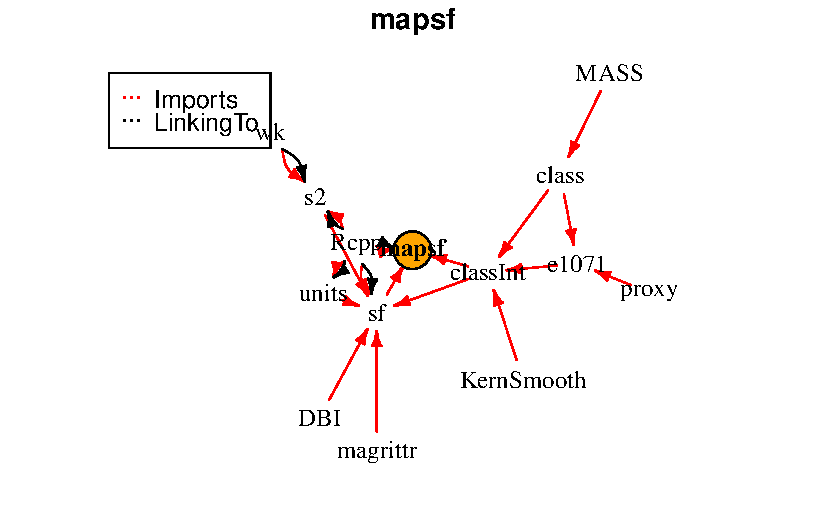
\includegraphics{minicran_files/figure-pdf/unnamed-chunk-3-1.pdf}

}

\end{figure}

\hypertarget{cruxe9er-son-minicran}{%
\subsubsection{\texorpdfstring{Créer son
\emph{miniCRAN}}{Créer son miniCRAN}}\label{cruxe9er-son-minicran}}

Avant d'importer les sources des packages ciblés ainsi que leurs
dépendances, créez un nouveau répertoire qui permettra de les stocker.
Vous pouvez le faire manuellement ou en code R avec la fonction
\texttt{dir.create()} :

\begin{Shaded}
\begin{Highlighting}[]
\NormalTok{path\_miniCRAN }\OtherTok{\textless{}{-}} \StringTok{"/home/hugues/Documents/5.Cours/Modules\_R/miniCRAN"}

\CommentTok{\# Création du répertoire nommé "miniCRAN"}
\FunctionTok{dir.create}\NormalTok{(}\AttributeTok{path =}\NormalTok{ path\_miniCRAN)}
\end{Highlighting}
\end{Shaded}

Il ne vous reste plus qu'à remplir votre répertoire avec les sources des
packages ciblés. Pour cela, utilisez la fonction \texttt{makeRepo()} :

\begin{Shaded}
\begin{Highlighting}[]
\CommentTok{\# Création d\textquotesingle{}un vecteur avec le ou les package(s) ciblé(s)}
\NormalTok{mes\_pkgs }\OtherTok{\textless{}{-}} \FunctionTok{c}\NormalTok{(}\StringTok{"readxl"}\NormalTok{, }\StringTok{"openxlsx"}\NormalTok{, }\StringTok{"haven"}\NormalTok{,}
              \StringTok{"dplyr"}\NormalTok{, }\StringTok{"lubridate"}\NormalTok{, }\StringTok{"stringr"}\NormalTok{,}
              \StringTok{"ggplot2"}\NormalTok{, }\StringTok{"FactoMineR"}\NormalTok{, }\StringTok{"sf"}\NormalTok{,}
              \StringTok{"terra"}\NormalTok{, }\StringTok{"mapsf"}\NormalTok{, }\StringTok{"rmarkdown"}\NormalTok{, }\StringTok{"knitr"}\NormalTok{)}


\CommentTok{\# Téléchargement des sources des packages (+ dépendances) dans le répertoire "miniCRAN"}
\FunctionTok{makeRepo}\NormalTok{(}\FunctionTok{pkgDep}\NormalTok{(mes\_pkgs), }\AttributeTok{path =}\NormalTok{ path\_miniCRAN, }\AttributeTok{type =} \FunctionTok{c}\NormalTok{(}\StringTok{"source"}\NormalTok{, }\StringTok{"mac.binary"}\NormalTok{, }\StringTok{"win.binary"}\NormalTok{))}
\end{Highlighting}
\end{Shaded}

\hypertarget{ajouter-des-packages}{%
\subsubsection{Ajouter des packages}\label{ajouter-des-packages}}

Il est très simple de rajouter de nouveaux packages (et leur
dépendances) dans votre \emph{miniCRAN} en utilisant la fonction
\texttt{addPackage()} :

\begin{Shaded}
\begin{Highlighting}[]
\FunctionTok{addPackage}\NormalTok{(}\StringTok{"tidyr"}\NormalTok{, }\AttributeTok{path =}\NormalTok{ path\_miniCRAN, }\AttributeTok{type =} \FunctionTok{c}\NormalTok{(}\StringTok{"source"}\NormalTok{, }\StringTok{"mac.binary"}\NormalTok{, }\StringTok{"win.binary"}\NormalTok{))}
\end{Highlighting}
\end{Shaded}

Pour lister l'ensemble des packages stockés sur votre \emph{miniCRAN},
utilisez la fonction \texttt{pkgAvail()} :

\begin{Shaded}
\begin{Highlighting}[]
\CommentTok{\# Check for available packages}
\FunctionTok{pkgAvail}\NormalTok{(}\AttributeTok{repos =}\NormalTok{ path\_miniCRAN, )[, }\FunctionTok{c}\NormalTok{(}\DecValTok{1}\SpecialCharTok{:}\DecValTok{3}\NormalTok{, }\DecValTok{5}\NormalTok{)]}
\end{Highlighting}
\end{Shaded}

\hypertarget{installer-un-package-du-minicran}{%
\subsubsection{Installer un package du
miniCRAN}\label{installer-un-package-du-minicran}}

Pour installer un package stocké sur votre \emph{miniCRAN} local,
utilisez la fonction \texttt{install.packages()}de la manière suivante :

\begin{Shaded}
\begin{Highlighting}[]
\CommentTok{\# Chemin d\textquotesingle{}accès jusqu\textquotesingle{}au "miniCRAN" stocké sur votre machine.}
\NormalTok{url\_miniCRAN }\OtherTok{\textless{}{-}} \FunctionTok{paste0}\NormalTok{(}\StringTok{"file:///"}\NormalTok{, }\StringTok{"C:/Users/\textless{}username\textgreater{}/.../miniCRAN"}\NormalTok{)}

\CommentTok{\# Installation de ggplot2 }
\FunctionTok{install.packages}\NormalTok{(}\StringTok{"ggplot2"}\NormalTok{, }
                 \AttributeTok{repos =}\NormalTok{ url\_miniCRAN,}
                 \AttributeTok{type =} \StringTok{"source"}\NormalTok{)}
\end{Highlighting}
\end{Shaded}

\hypertarget{le-minicran-de-tigr}{%
\subsubsection{Le miniCRAN de TIG'R}\label{le-minicran-de-tigr}}

Un \emph{miniCRAN} comportant l'ensemble des packages utilisés dans les
leçons de ce site web est mis à disposition. Vous pouvez le télécharger
en vous connectant à cette \href{https://bit.ly/3X1L4lk}{page}.

\hypertarget{pour-aller-plus-loin}{%
\subsubsection{Pour aller plus loin}\label{pour-aller-plus-loin}}

Pour connaitre l'ensemble des fonctionnalités offertes par le package
\texttt{miniCRAN}, consultez le
\href{http://andrie.github.io/miniCRAN/index.html}{site web du package}.

\hfill\break
\hfill\break



\end{document}
